% Generated by Sphinx.
\def\sphinxdocclass{report}
\documentclass[letterpaper,10pt,english]{sphinxmanual}
\usepackage[utf8]{inputenc}
\DeclareUnicodeCharacter{00A0}{\nobreakspace}
\usepackage{cmap}
\usepackage[T1]{fontenc}
\usepackage{babel}
\usepackage{times}
\usepackage[Bjarne]{fncychap}
\usepackage{longtable}
\usepackage{sphinx}
\usepackage{multirow}


\title{matchApp Documentation}
\date{June 23, 2016}
\release{2}
\author{Grupo5}
\newcommand{\sphinxlogo}{}
\renewcommand{\releasename}{Release}
\makeindex

\makeatletter
\def\PYG@reset{\let\PYG@it=\relax \let\PYG@bf=\relax%
    \let\PYG@ul=\relax \let\PYG@tc=\relax%
    \let\PYG@bc=\relax \let\PYG@ff=\relax}
\def\PYG@tok#1{\csname PYG@tok@#1\endcsname}
\def\PYG@toks#1+{\ifx\relax#1\empty\else%
    \PYG@tok{#1}\expandafter\PYG@toks\fi}
\def\PYG@do#1{\PYG@bc{\PYG@tc{\PYG@ul{%
    \PYG@it{\PYG@bf{\PYG@ff{#1}}}}}}}
\def\PYG#1#2{\PYG@reset\PYG@toks#1+\relax+\PYG@do{#2}}

\expandafter\def\csname PYG@tok@gd\endcsname{\def\PYG@tc##1{\textcolor[rgb]{0.63,0.00,0.00}{##1}}}
\expandafter\def\csname PYG@tok@gu\endcsname{\let\PYG@bf=\textbf\def\PYG@tc##1{\textcolor[rgb]{0.50,0.00,0.50}{##1}}}
\expandafter\def\csname PYG@tok@gt\endcsname{\def\PYG@tc##1{\textcolor[rgb]{0.00,0.27,0.87}{##1}}}
\expandafter\def\csname PYG@tok@gs\endcsname{\let\PYG@bf=\textbf}
\expandafter\def\csname PYG@tok@gr\endcsname{\def\PYG@tc##1{\textcolor[rgb]{1.00,0.00,0.00}{##1}}}
\expandafter\def\csname PYG@tok@cm\endcsname{\let\PYG@it=\textit\def\PYG@tc##1{\textcolor[rgb]{0.25,0.50,0.56}{##1}}}
\expandafter\def\csname PYG@tok@vg\endcsname{\def\PYG@tc##1{\textcolor[rgb]{0.73,0.38,0.84}{##1}}}
\expandafter\def\csname PYG@tok@m\endcsname{\def\PYG@tc##1{\textcolor[rgb]{0.13,0.50,0.31}{##1}}}
\expandafter\def\csname PYG@tok@mh\endcsname{\def\PYG@tc##1{\textcolor[rgb]{0.13,0.50,0.31}{##1}}}
\expandafter\def\csname PYG@tok@cs\endcsname{\def\PYG@tc##1{\textcolor[rgb]{0.25,0.50,0.56}{##1}}\def\PYG@bc##1{\setlength{\fboxsep}{0pt}\colorbox[rgb]{1.00,0.94,0.94}{\strut ##1}}}
\expandafter\def\csname PYG@tok@ge\endcsname{\let\PYG@it=\textit}
\expandafter\def\csname PYG@tok@vc\endcsname{\def\PYG@tc##1{\textcolor[rgb]{0.73,0.38,0.84}{##1}}}
\expandafter\def\csname PYG@tok@il\endcsname{\def\PYG@tc##1{\textcolor[rgb]{0.13,0.50,0.31}{##1}}}
\expandafter\def\csname PYG@tok@go\endcsname{\def\PYG@tc##1{\textcolor[rgb]{0.20,0.20,0.20}{##1}}}
\expandafter\def\csname PYG@tok@cp\endcsname{\def\PYG@tc##1{\textcolor[rgb]{0.00,0.44,0.13}{##1}}}
\expandafter\def\csname PYG@tok@gi\endcsname{\def\PYG@tc##1{\textcolor[rgb]{0.00,0.63,0.00}{##1}}}
\expandafter\def\csname PYG@tok@gh\endcsname{\let\PYG@bf=\textbf\def\PYG@tc##1{\textcolor[rgb]{0.00,0.00,0.50}{##1}}}
\expandafter\def\csname PYG@tok@ni\endcsname{\let\PYG@bf=\textbf\def\PYG@tc##1{\textcolor[rgb]{0.84,0.33,0.22}{##1}}}
\expandafter\def\csname PYG@tok@nl\endcsname{\let\PYG@bf=\textbf\def\PYG@tc##1{\textcolor[rgb]{0.00,0.13,0.44}{##1}}}
\expandafter\def\csname PYG@tok@nn\endcsname{\let\PYG@bf=\textbf\def\PYG@tc##1{\textcolor[rgb]{0.05,0.52,0.71}{##1}}}
\expandafter\def\csname PYG@tok@no\endcsname{\def\PYG@tc##1{\textcolor[rgb]{0.38,0.68,0.84}{##1}}}
\expandafter\def\csname PYG@tok@na\endcsname{\def\PYG@tc##1{\textcolor[rgb]{0.25,0.44,0.63}{##1}}}
\expandafter\def\csname PYG@tok@nb\endcsname{\def\PYG@tc##1{\textcolor[rgb]{0.00,0.44,0.13}{##1}}}
\expandafter\def\csname PYG@tok@nc\endcsname{\let\PYG@bf=\textbf\def\PYG@tc##1{\textcolor[rgb]{0.05,0.52,0.71}{##1}}}
\expandafter\def\csname PYG@tok@nd\endcsname{\let\PYG@bf=\textbf\def\PYG@tc##1{\textcolor[rgb]{0.33,0.33,0.33}{##1}}}
\expandafter\def\csname PYG@tok@ne\endcsname{\def\PYG@tc##1{\textcolor[rgb]{0.00,0.44,0.13}{##1}}}
\expandafter\def\csname PYG@tok@nf\endcsname{\def\PYG@tc##1{\textcolor[rgb]{0.02,0.16,0.49}{##1}}}
\expandafter\def\csname PYG@tok@si\endcsname{\let\PYG@it=\textit\def\PYG@tc##1{\textcolor[rgb]{0.44,0.63,0.82}{##1}}}
\expandafter\def\csname PYG@tok@s2\endcsname{\def\PYG@tc##1{\textcolor[rgb]{0.25,0.44,0.63}{##1}}}
\expandafter\def\csname PYG@tok@vi\endcsname{\def\PYG@tc##1{\textcolor[rgb]{0.73,0.38,0.84}{##1}}}
\expandafter\def\csname PYG@tok@nt\endcsname{\let\PYG@bf=\textbf\def\PYG@tc##1{\textcolor[rgb]{0.02,0.16,0.45}{##1}}}
\expandafter\def\csname PYG@tok@nv\endcsname{\def\PYG@tc##1{\textcolor[rgb]{0.73,0.38,0.84}{##1}}}
\expandafter\def\csname PYG@tok@s1\endcsname{\def\PYG@tc##1{\textcolor[rgb]{0.25,0.44,0.63}{##1}}}
\expandafter\def\csname PYG@tok@gp\endcsname{\let\PYG@bf=\textbf\def\PYG@tc##1{\textcolor[rgb]{0.78,0.36,0.04}{##1}}}
\expandafter\def\csname PYG@tok@sh\endcsname{\def\PYG@tc##1{\textcolor[rgb]{0.25,0.44,0.63}{##1}}}
\expandafter\def\csname PYG@tok@ow\endcsname{\let\PYG@bf=\textbf\def\PYG@tc##1{\textcolor[rgb]{0.00,0.44,0.13}{##1}}}
\expandafter\def\csname PYG@tok@sx\endcsname{\def\PYG@tc##1{\textcolor[rgb]{0.78,0.36,0.04}{##1}}}
\expandafter\def\csname PYG@tok@bp\endcsname{\def\PYG@tc##1{\textcolor[rgb]{0.00,0.44,0.13}{##1}}}
\expandafter\def\csname PYG@tok@c1\endcsname{\let\PYG@it=\textit\def\PYG@tc##1{\textcolor[rgb]{0.25,0.50,0.56}{##1}}}
\expandafter\def\csname PYG@tok@kc\endcsname{\let\PYG@bf=\textbf\def\PYG@tc##1{\textcolor[rgb]{0.00,0.44,0.13}{##1}}}
\expandafter\def\csname PYG@tok@c\endcsname{\let\PYG@it=\textit\def\PYG@tc##1{\textcolor[rgb]{0.25,0.50,0.56}{##1}}}
\expandafter\def\csname PYG@tok@mf\endcsname{\def\PYG@tc##1{\textcolor[rgb]{0.13,0.50,0.31}{##1}}}
\expandafter\def\csname PYG@tok@err\endcsname{\def\PYG@bc##1{\setlength{\fboxsep}{0pt}\fcolorbox[rgb]{1.00,0.00,0.00}{1,1,1}{\strut ##1}}}
\expandafter\def\csname PYG@tok@mb\endcsname{\def\PYG@tc##1{\textcolor[rgb]{0.13,0.50,0.31}{##1}}}
\expandafter\def\csname PYG@tok@ss\endcsname{\def\PYG@tc##1{\textcolor[rgb]{0.32,0.47,0.09}{##1}}}
\expandafter\def\csname PYG@tok@sr\endcsname{\def\PYG@tc##1{\textcolor[rgb]{0.14,0.33,0.53}{##1}}}
\expandafter\def\csname PYG@tok@mo\endcsname{\def\PYG@tc##1{\textcolor[rgb]{0.13,0.50,0.31}{##1}}}
\expandafter\def\csname PYG@tok@kd\endcsname{\let\PYG@bf=\textbf\def\PYG@tc##1{\textcolor[rgb]{0.00,0.44,0.13}{##1}}}
\expandafter\def\csname PYG@tok@mi\endcsname{\def\PYG@tc##1{\textcolor[rgb]{0.13,0.50,0.31}{##1}}}
\expandafter\def\csname PYG@tok@kn\endcsname{\let\PYG@bf=\textbf\def\PYG@tc##1{\textcolor[rgb]{0.00,0.44,0.13}{##1}}}
\expandafter\def\csname PYG@tok@o\endcsname{\def\PYG@tc##1{\textcolor[rgb]{0.40,0.40,0.40}{##1}}}
\expandafter\def\csname PYG@tok@kr\endcsname{\let\PYG@bf=\textbf\def\PYG@tc##1{\textcolor[rgb]{0.00,0.44,0.13}{##1}}}
\expandafter\def\csname PYG@tok@s\endcsname{\def\PYG@tc##1{\textcolor[rgb]{0.25,0.44,0.63}{##1}}}
\expandafter\def\csname PYG@tok@kp\endcsname{\def\PYG@tc##1{\textcolor[rgb]{0.00,0.44,0.13}{##1}}}
\expandafter\def\csname PYG@tok@w\endcsname{\def\PYG@tc##1{\textcolor[rgb]{0.73,0.73,0.73}{##1}}}
\expandafter\def\csname PYG@tok@kt\endcsname{\def\PYG@tc##1{\textcolor[rgb]{0.56,0.13,0.00}{##1}}}
\expandafter\def\csname PYG@tok@sc\endcsname{\def\PYG@tc##1{\textcolor[rgb]{0.25,0.44,0.63}{##1}}}
\expandafter\def\csname PYG@tok@sb\endcsname{\def\PYG@tc##1{\textcolor[rgb]{0.25,0.44,0.63}{##1}}}
\expandafter\def\csname PYG@tok@k\endcsname{\let\PYG@bf=\textbf\def\PYG@tc##1{\textcolor[rgb]{0.00,0.44,0.13}{##1}}}
\expandafter\def\csname PYG@tok@se\endcsname{\let\PYG@bf=\textbf\def\PYG@tc##1{\textcolor[rgb]{0.25,0.44,0.63}{##1}}}
\expandafter\def\csname PYG@tok@sd\endcsname{\let\PYG@it=\textit\def\PYG@tc##1{\textcolor[rgb]{0.25,0.44,0.63}{##1}}}

\def\PYGZbs{\char`\\}
\def\PYGZus{\char`\_}
\def\PYGZob{\char`\{}
\def\PYGZcb{\char`\}}
\def\PYGZca{\char`\^}
\def\PYGZam{\char`\&}
\def\PYGZlt{\char`\<}
\def\PYGZgt{\char`\>}
\def\PYGZsh{\char`\#}
\def\PYGZpc{\char`\%}
\def\PYGZdl{\char`\$}
\def\PYGZhy{\char`\-}
\def\PYGZsq{\char`\'}
\def\PYGZdq{\char`\"}
\def\PYGZti{\char`\~}
% for compatibility with earlier versions
\def\PYGZat{@}
\def\PYGZlb{[}
\def\PYGZrb{]}
\makeatother

\renewcommand\PYGZsq{\textquotesingle}

\begin{document}

\maketitle
\tableofcontents
\phantomsection\label{index::doc}


Contenidos:


\chapter{Manual de programador - Documentación Técnica}
\label{manuals::doc}\label{manuals:manual-de-programador-documentacion-tecnica}\label{manuals:documentacion-de-matchapp}
\textbf{Grupo 10}

\textbf{Ayudante asignado: Christian Calonico}

\textbf{Integrantes:}

\begin{tabulary}{\linewidth}{|L|L|}
\hline
\textsf{\relax 
Apellido y Nombre
} & \textsf{\relax 
Padrón
}\\
\hline
Daye, Gisela Denise
 & 
87602
\\
\hline
Federico, Pablo
 & 
90280
\\
\hline
Farina, Federico
 & 
90177
\\
\hline
Vazquez, Nicolás
 & 
89172
\\
\hline\end{tabulary}



\section{Tecnologías utilizadas}
\label{manuals:tecnologias-utilizadas}

\subsection{Cliente}
\label{manuals:cliente}\begin{itemize}
\item {} 
Android SDK compatible hasta v23

\item {} 
Volley

\item {} 
Material Design para templates

\end{itemize}


\subsection{Application Server}
\label{manuals:application-server}\begin{itemize}
\item {} 
Cmake

\item {} 
CI-Travis

\item {} 
Mongoose-cpp

\item {} 
Jsoncpp

\item {} 
Casablanca

\item {} 
RocksDB (v4.4.1)

\item {} 
Docker

\item {} 
Code coverage con gcov

\item {} 
Unit tests (cppunit)

\item {} 
Tests de endpoints con Postman

\item {} 
Tests funcionales con Python (pip y requests)

\end{itemize}


\subsection{Shared Server}
\label{manuals:shared-server}\begin{itemize}
\item {} 
Utilización de Heroku, para hostear la base de datos y la aplicación web.

\end{itemize}

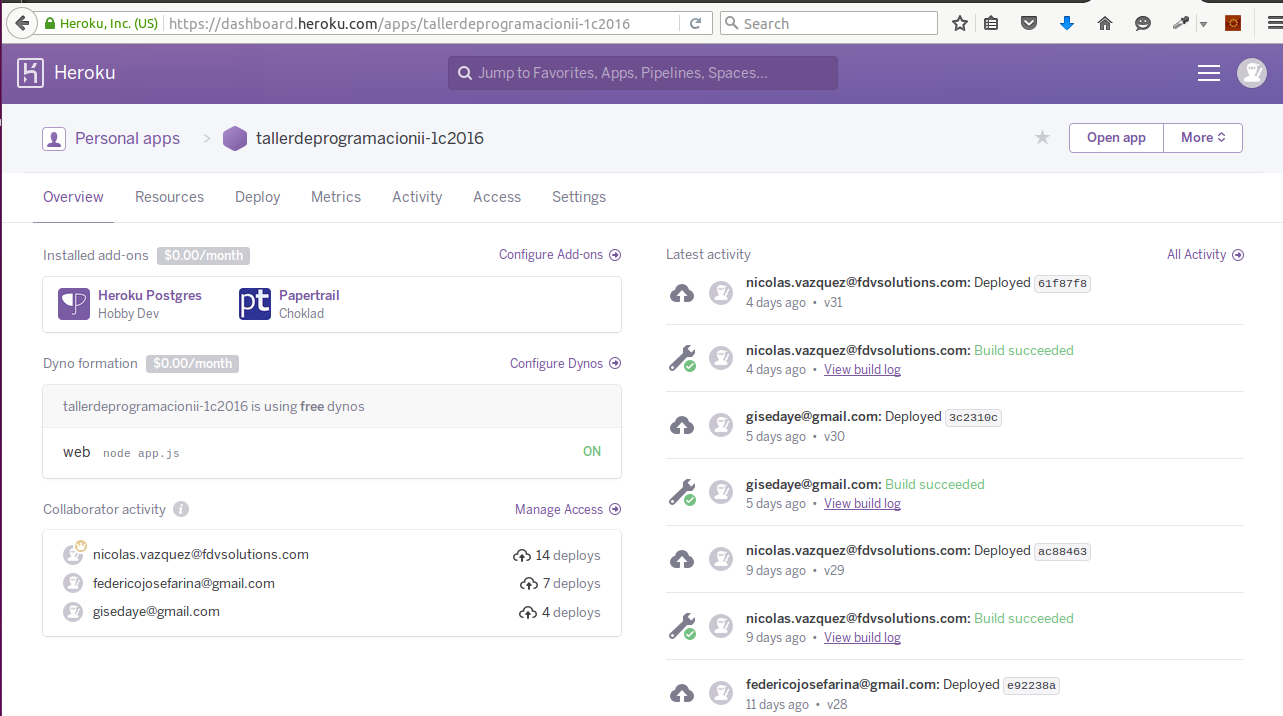
\includegraphics{heroku.png}
\begin{itemize}
\item {} 
Utilización de Express + Node.js en sus versiones 4.13 y 0.12.7 respectivamente.

\item {} 
Utilización de una base de datos PostgreSQL para almacenamiento de la información de Match App.

\end{itemize}

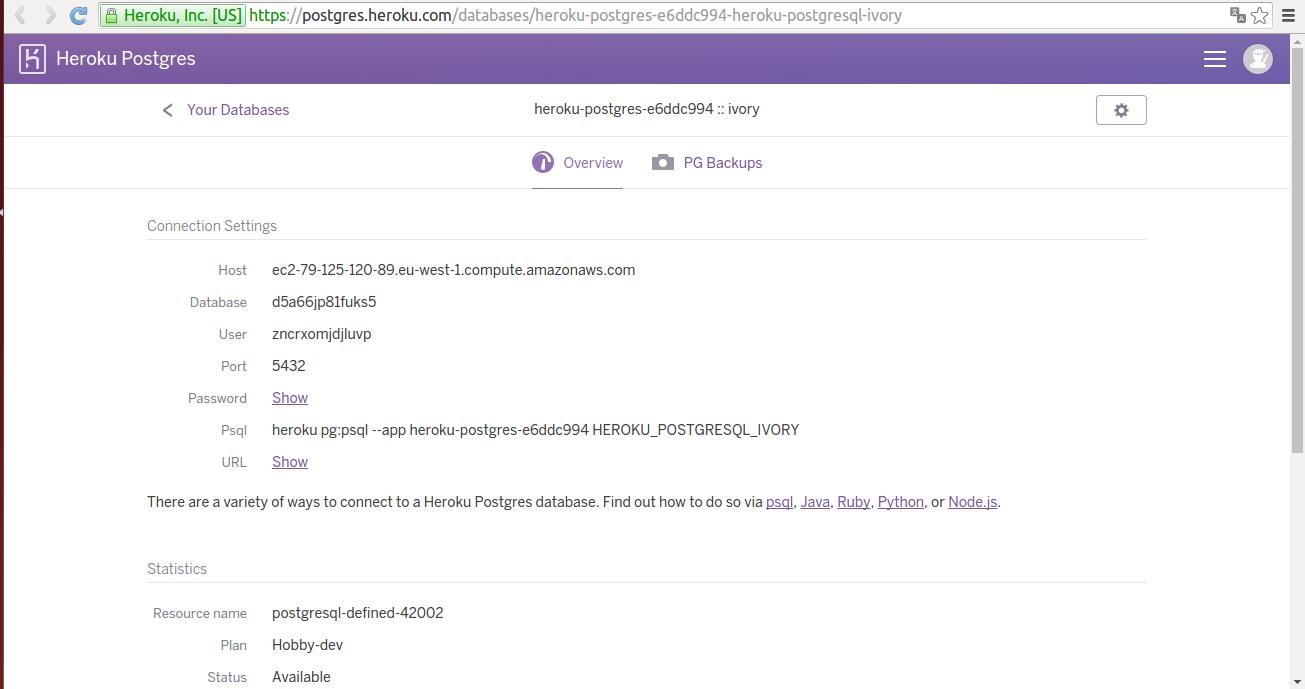
\includegraphics{postgresql.png}
\begin{itemize}
\item {} 
Aplicación Web utilizando CSS, HTML, Boostrap + Materialize, JQuery y Ajax.

\item {} 
Test  de endpoints con Postman

\item {} 
Docker

\end{itemize}


\subsection{Proyecto}
\label{manuals:proyecto}
-- Documentación en Sphinx
- Utilización de 3 repositorios en GitHub. (Cliente, App Server y Shared Server)
- Shared Server: \href{https://github.com/PabloFederico/SharedServer}{https://github.com/PabloFederico/SharedServer}
- App Server: \href{https://github.com/nicolas-vazquez/tp75521c}{https://github.com/nicolas-vazquez/tp75521c}
- Cliente y Documentación: \href{https://github.com/gisedaye/taller2android}{https://github.com/gisedaye/taller2android}


\section{Arquitectura}
\label{manuals:arquitectura}
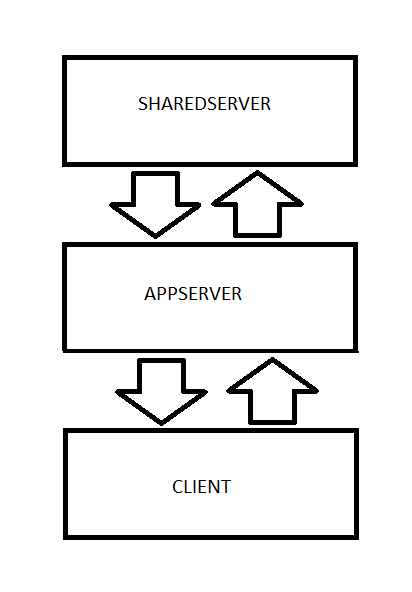
\includegraphics{architecture.png}


\subsection{Appserver}
\label{manuals:appserver}

\subsubsection{Esquemas}
\label{manuals:esquemas}
Paquetes del appServer

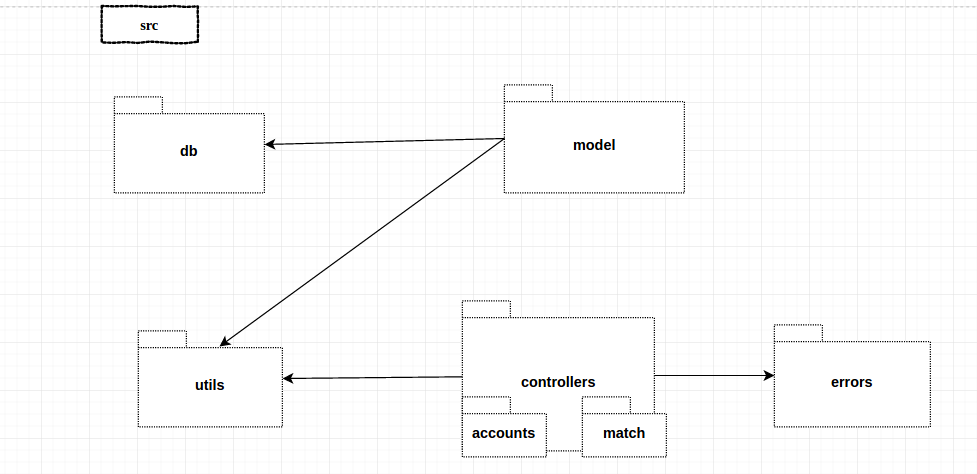
\includegraphics{Screenshots/paquetesApp.png}

Modelos y Controladores básicos del sistema.

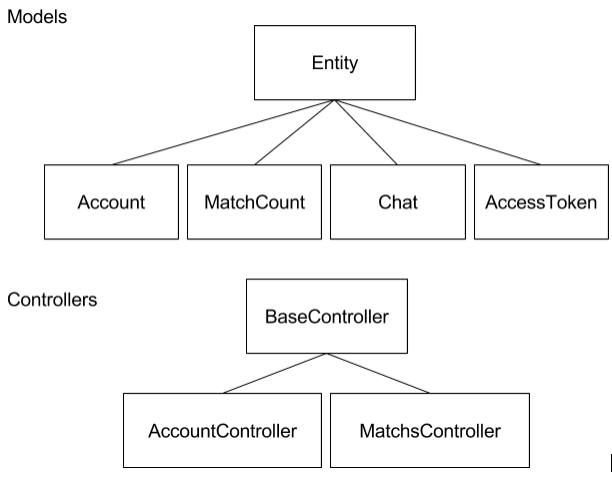
\includegraphics{classesapp.png}

Esquemas de la base de datos de rocksDB.

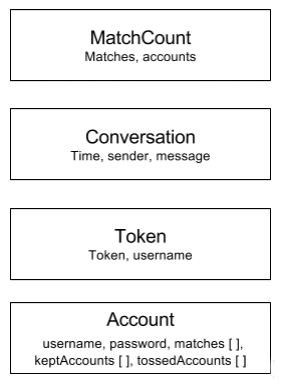
\includegraphics{rocksdb.png}

Diagrama de secuencia

..image:: Screenshots/secuenciaAppMain.png


\subsubsection{Endpoints}
\label{manuals:endpoints}
A continuación se brindará una breve descripción de los distintos endpoints del App Server y como se manejan para obtener la información.


\subsubsection{Signup}
\label{manuals:signup}\begin{itemize}
\item {} 
Desde el cliente se realiza un request a App Server con los datos del profile e intereses completos.

\item {} 
Se almacena username y password en el App Server.

\item {} 
Se realiza un request a Shared Server para crear un usuario con los datos restantes (profile e intereses).

\item {} 
Se almacena la información del profile en Shared Server.

\item {} 
Se retorna la respuesta con un mensaje de error en caso de fallo o con un mensaje exitoso en caso contrario.

\end{itemize}


\subsubsection{Login}
\label{manuals:login}\begin{itemize}
\item {} 
Desde el cliente se realiza un request a App Server con username/password.

\item {} 
Se corrobora si existe el usuario en la base de datos de App Server.

\item {} 
En el caso que exista se realiza un request a Shared Server para obtener el profile del usuario que luego de retorna junto con el Access Token.

\item {} 
Si no existe se realiza un request a Shared Server, ya que el usuario puede haber sido creado desde el backoffice.

\item {} 
Se busca el usuario en el Shared Server y si existe se devuelve el profile. En caso que no exista se devuelve un error al App Server.

\item {} 
Si hubo error se devuelve un mensaje de error a la aplicación Cliente. En caso contrario se guarda username/password en el AppServer.

\item {} 
Se retorna la respuesta con el Access Token y el profile del usuario.

\end{itemize}


\subsubsection{Like/Dislike}
\label{manuals:like-dislike}\begin{itemize}
\item {} 
Desde el cliente se realiza un request a App Server con el id del usuario elegido como parámetro.

\item {} 
Se almacena el id en el array de keptAccounts.

\item {} 
En caso de producirse un match se almacena el mismo.

\end{itemize}


\subsubsection{Get Candidates}
\label{manuals:get-candidates}\begin{itemize}
\item {} 
Desde el cliente se realiza un request a App Server con los datos de la localización geográfica del usuario.

\item {} 
Se corrobora si existe el usuario en la base de datos de App Server.

\item {} 
Se realiza un request a SharedServer con el alias del usuario para obtener los candidatos que compartan algún interés con el usuario y se encuentren dentro del radio de localización correspondiente.

\item {} 
Shared Server determina los candidatos de acuerdo a los intereses del usuario.

\item {} 
Se retornan la respuesta con los perfiles de los candidatos al App Server y se filtra por likes/dislikes.

\item {} 
Se devuelve un candidato que cumpla con los requisitos de compartir un interés con el usuario, encontrarse dentro del radio de localización correspondiente y poseer una cantidad de matches menor al 1\% del total de matches por usuario promedio.

\end{itemize}


\subsubsection{Get Matches}
\label{manuals:get-matches}\begin{itemize}
\item {} 
Desde el cliente se realiza un request al App Server.

\item {} 
Se obtiene la lista de matches asociados al usuario.

\item {} 
Se realiza un request a Shared Server con el listado de matches para obtener los profiles asociados a los mismos.

\item {} 
Se retorna la respuesta a la aplicación Cliente con los datos de los usuarios que poseen un match con el usuario.

\end{itemize}


\subsection{Sharedserver}
\label{manuals:sharedserver}

\subsubsection{Esquemas}
\label{manuals:id1}\begin{itemize}
\item {} 
A continuación se mostrará un esquema de funcionamiento del Shared Sever, para poder explicar el flujo en la utilización de la API

\end{itemize}

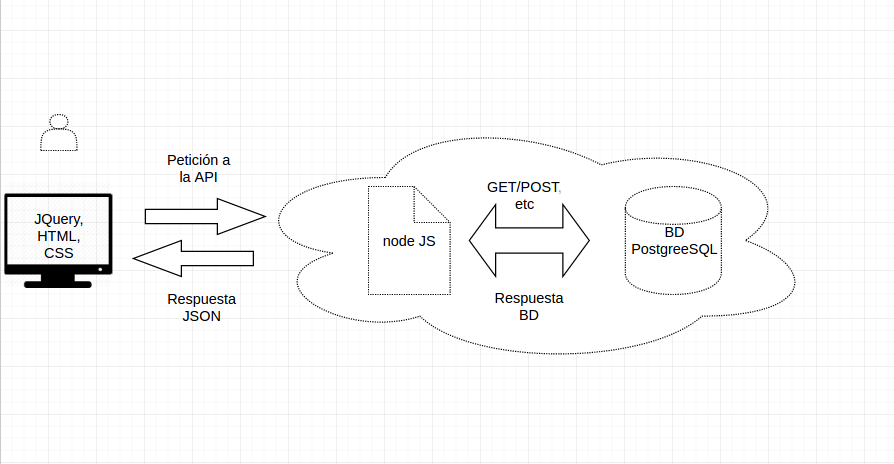
\includegraphics{esquemaShared.png}
\begin{itemize}
\item {} 
En el siguiente Diagrama de Componentes podemos visualizar la interacción entre los diferentes módulos de Shared Server. Por un lado, todas las dependencias necesarias para el funcionamiento se encuentran dentro de node\_modules. En la parte central se encuentra el servidor, que tiene interacción con las dependencias de la aplicación, con las vistas y con la API. En el caso de la API, interactúa con las vistas y con el servidor para enviar la respuesta a las solicitudes del mismo.

\end{itemize}

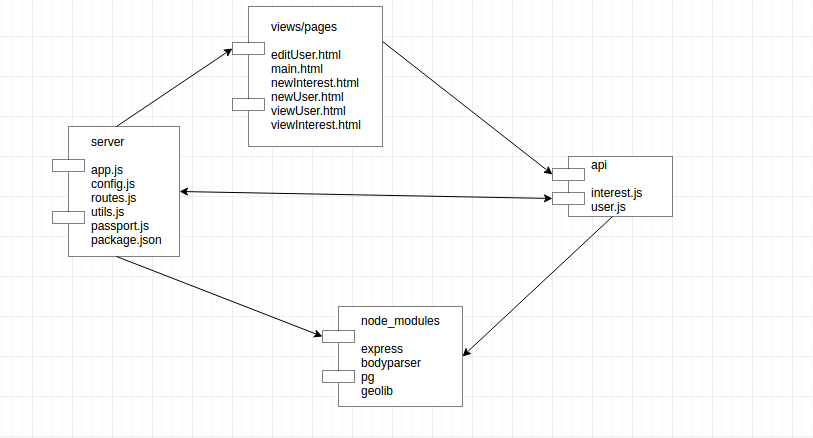
\includegraphics{Screenshots/componentes3Shared.png}
\begin{itemize}
\item {} 
Se crearon tres tablas en la base de datos de PostgreSQL para almacenar la información de los usuarios y sus intereses. EL esquema de tablas utilizados es el siguiente

\end{itemize}

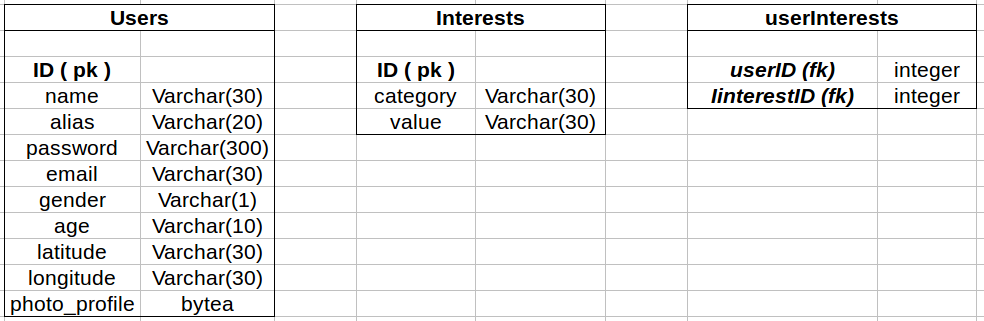
\includegraphics{tablasShared.png}
\begin{itemize}
\item {} 
El siguiente es un Diagrama Entidad-Relación de la base de datos:

\end{itemize}

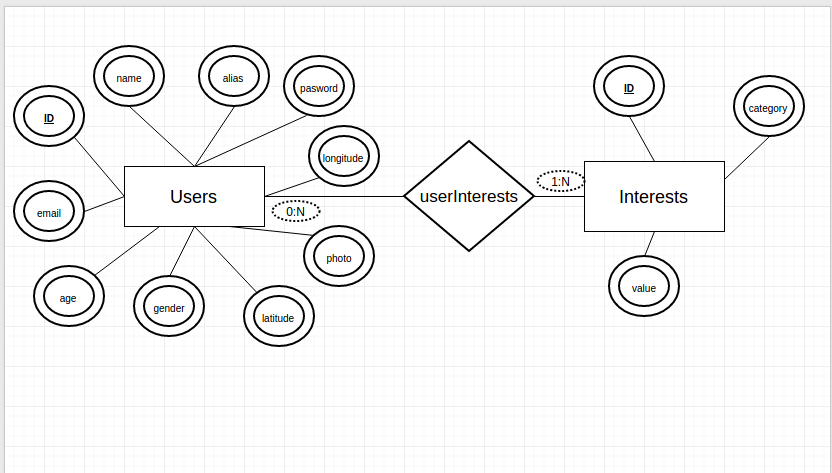
\includegraphics{Screenshots/derShared.png}


\subsubsection{Listado de usuarios}
\label{manuals:listado-de-usuarios}\begin{itemize}
\item {} 
Request GET /users

\item {} 
Devuelve un listado de usuarios con: id, name, alias, email, sex, age, photo\_profile, interests, location, metadata

\end{itemize}


\subsubsection{Alta de usuario}
\label{manuals:alta-de-usuario}\begin{itemize}
\item {} 
Request POST /users con parámetros: name, alias, email, sex, age, interests, location, photo\_profile

\item {} 
Crea el usuario en el Shared Server

\end{itemize}


\subsubsection{Consulta perfil de usuario}
\label{manuals:consulta-perfil-de-usuario}\begin{itemize}
\item {} 
Request GET /users/:id

\item {} 
Busca en el Shared Server un usuario con el id correspondiente a la solicitud

\item {} 
Devuelve un error en caso que no exista o en caso contrario un usuario con las siguientes propiedades: id, name, alias, email, sex, age, photo\_profile, array de interests, location, metadata

\end{itemize}


\subsubsection{Edición de usuario}
\label{manuals:edicion-de-usuario}\begin{itemize}
\item {} 
Request PUT /users/:id con parámetros: id, name, alias, email, sex, age, photo\_profile, interests, location

\item {} 
Modifica el perfil del usuario en el Shared Server y retorna un error en caso que haya ocurrido un fallo o un mensaje exitoso en caso contrario.

\end{itemize}


\subsubsection{Consulta foto de perfil}
\label{manuals:consulta-foto-de-perfil}\begin{itemize}
\item {} 
Request GET /users/:id/photo con parámetro: id del usuario

\item {} 
Obtiene la foto de perfil del usuario con el id correspondiente a la solicitud o un error en caso que no exista el usuario.

\end{itemize}


\subsubsection{Baja de usuario}
\label{manuals:baja-de-usuario}\begin{itemize}
\item {} 
Request DELETE /users/:id

\item {} 
Elimina al usuario del Shared Server y retorna un error en caso que haya ocurrido un fallo o un mensaje exitoso en caso contrario.

\end{itemize}


\subsubsection{Listado de intereses}
\label{manuals:listado-de-intereses}\begin{itemize}
\item {} 
Request GET /interests

\item {} 
Obtiene un listado con los intereses globales del Shared Server con las propiedades category y value o un error en caso que haya ocurrido un fallo.

\end{itemize}


\subsubsection{Alta de interés}
\label{manuals:alta-de-interes}\begin{itemize}
\item {} 
Request POST /interests con parametros: category, value

\item {} 
Crea un nuevo interés en el Shared Server para la categoría y valor correspondientes.

\end{itemize}


\subsection{Client}
\label{manuals:client}\begin{itemize}
\item {} 
Consume los servicios del App Server para Login, Registro, Búsqueda de Candidatos, Matches, Like, Dislike y Chat

\item {} 
Maneja una sesión con el Authorization Token provisto previamente por el Login

\item {} \begin{description}
\item[{Vistas:}] \leavevmode\begin{itemize}
\item {} 
LoginActivity

\item {} 
RegisterActivity

\item {} 
MainActivity

\item {} 
SplashActivity

\end{itemize}

\end{description}

\end{itemize}


\section{Testing}
\label{manuals:testing}

\subsection{Appserver}
\label{manuals:id2}

\subsubsection{Unit Tests}
\label{manuals:unit-tests}
En la consola desde la carpeta build ejecutar el comando
\begin{quote}

\textgreater{} ctest
\end{quote}


\subsubsection{Coverage}
\label{manuals:coverage}
En el directorio raíz del proyecto ejecutar el siguiente comando:
\begin{quote}

\textgreater{} sudo ./coverage.sh
\end{quote}

Se abrirá una ventana del navegador con los resultados del test coverage

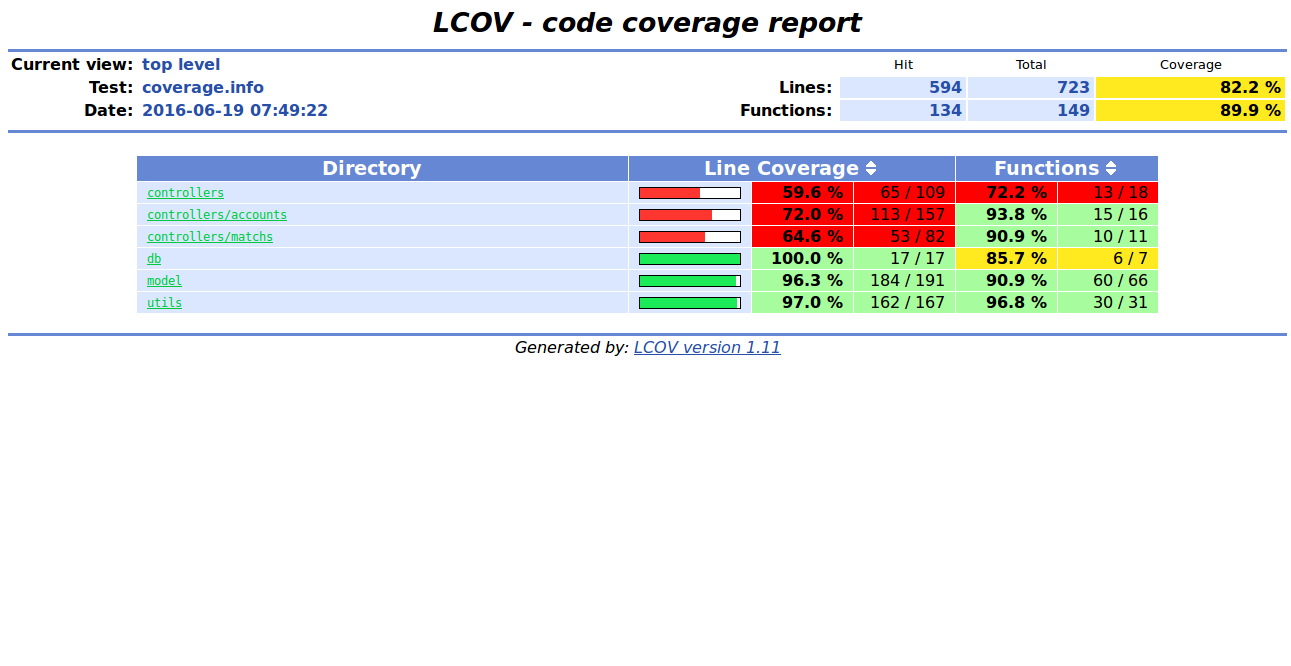
\includegraphics{coverage.png}


\subsubsection{Tests funcionales}
\label{manuals:tests-funcionales}
Instalar python

\textgreater{} sudo apt-get install python2.7

Instalar pip

\textgreater{} wget \href{https://bootstrap.pypa.io/get-pip.py}{https://bootstrap.pypa.io/get-pip.py}
\textgreater{} sudo python get-pip.py

Instalar el módulo requests

\textgreater{} sudo pip install requests

Para correr los tests funcionales dirigirse al directorio functionalTests y ejecutar los siguientes comandos:

\textgreater{} cd functionalTests/
\textgreater{} python python restTester.py

Se mostrarán los resultados de los tests en la consola


\subsubsection{Testear Endpoints Manualmente}
\label{manuals:testear-endpoints-manualmente}
Ejecutar el App Server (Ver Manual de instalación)
Ejecutar el cliente Postman


\subsubsection{SignUp}
\label{manuals:id3}
\code{POST http://127.0.0.1:8083/api/accounts/signup}

En la pestaña body, seleccionar el radiobutton raw y agregar el siguiente texto:

\code{\{
"username": "user",
"password": "P4ssw0rd"
\}}


\subsubsection{Login}
\label{manuals:id4}
\code{POST http://127.0.0.1:8083/api/accounts/login}

En la pestaña body, seleccionar el radiobutton raw y agregar el siguiente texto:

\code{\{
"username": "user",
"password": "P4ssw0rd"
\}}


\subsubsection{Matches}
\label{manuals:matches}
\code{GET http://127.0.0.1:8083/api/matches/}

Setear el header Authorization con el token que se recibió en la solicitud de Login

\code{Authorization: \textless{}token\textgreater{}}


\subsubsection{Candidates}
\label{manuals:candidates}
\code{GET http://127.0.0.1:8083/api/matches/candidates}

Setear el header Authorization con el token que se recibió en la solicitud de Login

\code{Authorization: \textless{}token\textgreater{}}


\subsubsection{Ver mensajes}
\label{manuals:ver-mensajes}
\code{GET http://127.0.0.1:8083/api/matches/:id/messages}

Setear el header Authorization con el token que se recibió en la solicitud de Login

\code{Authorization: \textless{}token\textgreater{}}


\subsubsection{Enviar mensaje}
\label{manuals:enviar-mensaje}
\code{PUT http://127.0.0.1:8083/api/matches/:id/message}

\code{\{
"message": "Hola!"
\}}

Setear el header Authorization con el token que se recibió en la solicitud de Login

\code{Authorization: \textless{}token\textgreater{}}


\subsubsection{Like}
\label{manuals:like}
\code{PUT http://127.0.0.1:8083/api/accounts/:id/like}

Setear el header Authorization con el token que se recibió en la solicitud de Login

\code{Authorization: \textless{}token\textgreater{}}


\subsubsection{Disike}
\label{manuals:disike}
\code{PUT http://127.0.0.1:8083/api/accounts/:id/dislike}

Setear el header Authorization con el token que se recibió en la solicitud de Login

\code{Authorization: \textless{}token\textgreater{}}


\subsection{Shared Server}
\label{manuals:id5}

\subsubsection{Login}
\label{manuals:id6}
\code{POST http://127.0.0.1:8083/api/accounts/login}

En la pestaña body, seleccionar el radiobutton raw y agregar el siguiente texto

\code{\{
"username": "user",
"password": "P4ssw0rd"
\}}

Agregar headers

\code{Authorization: \textless{}token\textgreater{}}
\code{Content-Type: application/json}


\subsubsection{Listado de  usuarios}
\label{manuals:id7}
\code{GET https://tallerdeprogramacionii-1c2016.herokuapp.com/users}


\subsubsection{Vista de un usuario}
\label{manuals:vista-de-un-usuario}
\code{GET https://tallerdeprogramacionii-1c2016.herokuapp.com/users/:id}


\subsubsection{Consulta de perfil de usuario}
\label{manuals:consulta-de-perfil-de-usuario}
\code{GET https://tallerdeprogramacionii-1c2016.herokuapp.com/users/:id/profile}

Agregar headers

\code{Authorization: \textless{}token\textgreater{}}
\code{Content-Type: application/json}


\subsubsection{Consulta de candidatos para un usuario}
\label{manuals:consulta-de-candidatos-para-un-usuario}
\code{GET https://tallerdeprogramacionii-1c2016.herokuapp.com/users/:user/candidates}

Agregar headers

\code{Authorization: \textless{}token\textgreater{}}
\code{Content-Type: application/json}


\subsubsection{Alta de usuario}
\label{manuals:id8}
\code{POST https://tallerdeprogramacionii-1c2016.herokuapp.com/users}

\code{\{
"name":"Name",
"Alias":"aliiaass",
"age":23,
"gender":"M",
"email":"mail@mail.com",
"latitude":"-34.58",
"longitude":"-58.60",
"photo\_profile": "base\_64"
\}}


\subsubsection{Modificación de usuario}
\label{manuals:modificacion-de-usuario}
\code{PUT https://tallerdeprogramacionii-1c2016.herokuapp.com/users/:id}

\code{\{
"id": 1,
"name":"Name",
"Alias":"aliiaass",
"age":23,
"gender":"M",
"email":"mail@mail.com",
"latitude":"-34.58",
"longitude":"-58.60",
"photo\_profile": "base\_64"
\}}


\subsubsection{Baja de usuario}
\label{manuals:id9}
\code{DELETE https://tallerdeprogramacionii-1c2016.herokuapp.com/users/:id}


\subsubsection{Listado de intereses}
\label{manuals:id10}
\code{GET https://tallerdeprogramacionii-1c2016.herokuapp.com/interests}


\subsubsection{Alta de interés}
\label{manuals:id11}
\code{POST https://tallerdeprogramacionii-1c2016.herokuapp.com/interests}

\code{\{
"category":"Music",
"value":"One Direction"
\}}


\subsubsection{Baja de interés}
\label{manuals:baja-de-interes}
\code{DELETE https://tallerdeprogramacionii-1c2016.herokuapp.com/interests/:id}


\chapter{Indices y tablas}
\label{index:indices-y-tablas}\begin{itemize}
\item {} 
\emph{genindex}

\item {} 
\emph{modindex}

\item {} 
\emph{search}

\end{itemize}



\renewcommand{\indexname}{Index}
\printindex
\end{document}
